\chapter{Gamma-Ray Astronomy}
\label{ch:gamma-ray-astronomy}

Astronomy, being one of the oldest sciences, is a vast field of study dating back to the earliest
days of civilization, where astronomers have been studying the stars and the planets to understand
the universe. It, therefore, is no surprise that astronomy spawned a great number of discoveries
throughout the centuries. Whereas first observations were made by eye only, we now have access to a multitude
of experiments and telescopes that deepen our understanding of the universe. With the discovery of
\gls{cr} by Victor Hess in the early \nth{20} century, the new field of astroparticle physics was born \cite{longair1981}.

\begin{figure}
    \centering
    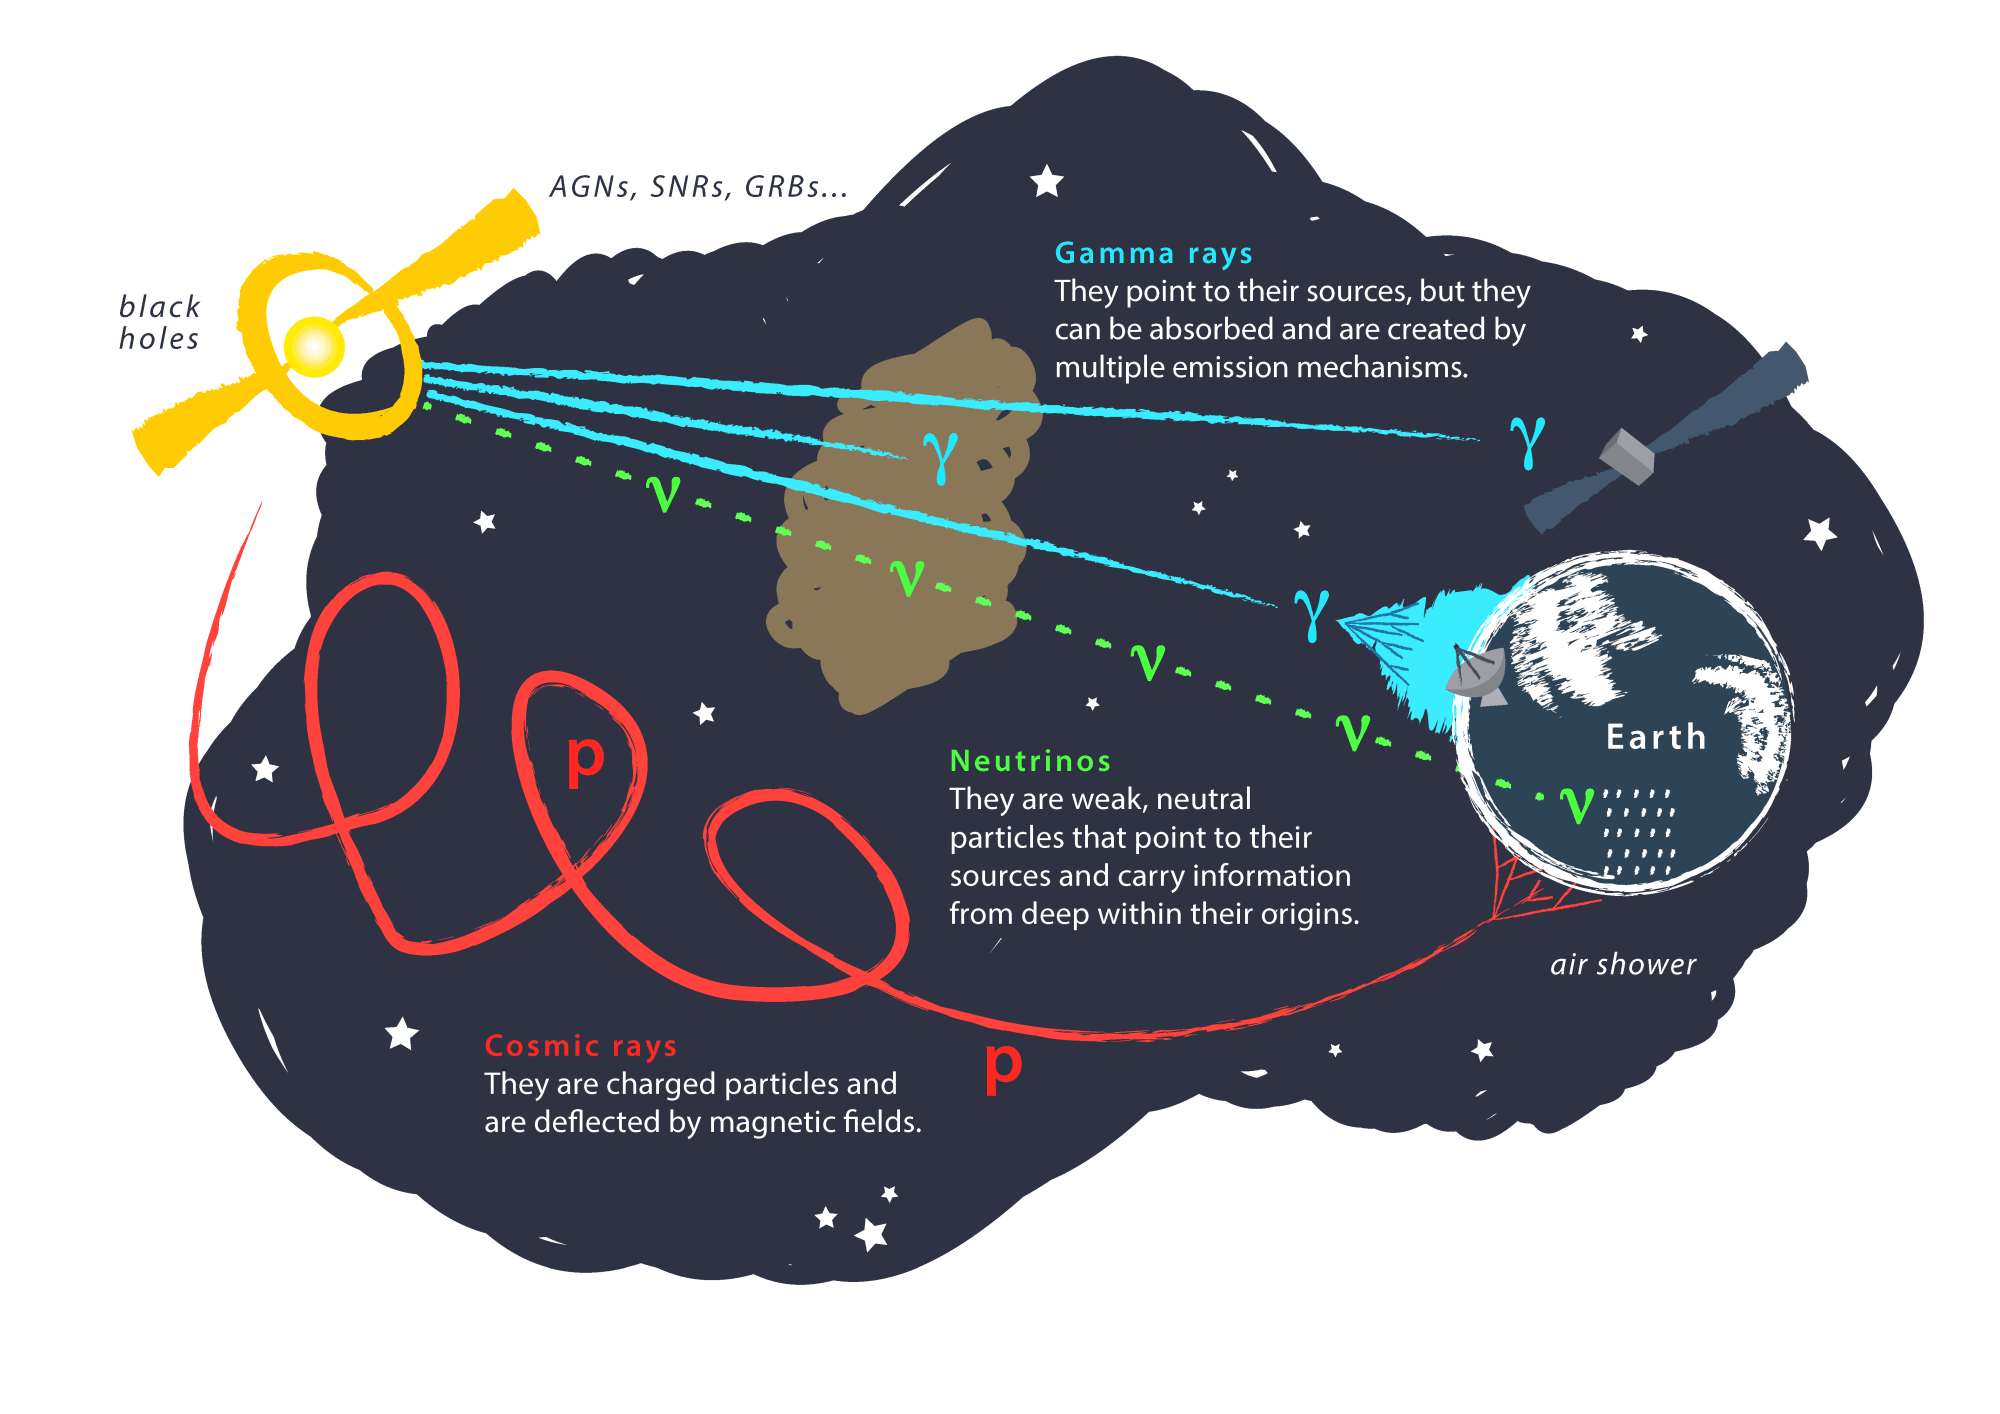
\includegraphics[width=0.8\textwidth]{graphics/figure5.png}
    \caption{Different types of cosmic messengers on their way to Earth. Charged particles like protons and electrons
    are deflected by magnetic fields and therefore making it hard to pinpoint the source. Only the
    origin of photons and neutrinos can be reconstructed directly since they are uncharged particles
    and therefore travel in straight lines. However, photons can be absorbed or created in multiple
    mechanisms. Since neutrinos only rarely interact with matter via the weak force, their detection
    is significantly harder than for photons \cite{fig5}.}
    \label{fig:fig5}
\end{figure}

Only \(\num{50}\) years after Hess' discovery, in 1961, Explorer XI \cite{explorer11}, the first satellite experiment
to measure gamma rays from space was launched, providing measurements of gamma rays above
\SI{50}{\mega\eV}, thus starting gamma-ray astronomy from space-based experiments. Just a few years
earlier neutrinos were already discovered by Cowan and Reines \cite{cowan1956}, with solar neutrinos being
discovered by Davis \etal{} \cite{davis} in the 1960s at the Homestake experiment.
The first detection of neutrinos from a supernova was made by the Kamiokande experiment in 1987
\cite{kamiokande1987}. The most recent discovery of a cosmic messenger has been that of gravitational
waves in 2015 \cite{grav_waves}.

Cosmic messengers come in different types, that are either charged or uncharged, as shown in \autoref{fig:fig5}.
\gls{cr} like electrons, protons or atomic nuclei are charged particles making it difficult to trace back their origin
as they are deflected by the cosmic electromagnetic fields. Uncharged particles like photons or
neutrinos, however, travel in straight lines, making it easier to reconstruct their origins.

While photons can be absorbed by dust clouds on their way to Earth, they are easier to detect than
neutrinos, the latter interacting only weakly with matter due to their small cross-section.
This means that neutrino detectors and experiments, such as IceCube \cite{icecube_2006} or
Super-Kamiokande \cite{kamiokande}, have to be large enough to detect the neutrinos in sufficient quantities.

In recent years, gamma-ray astronomy has become an important research field in astroparticle physics.
The term gamma ray is generally denoted as photons with energies above \SI{100}{\kilo\eV}
\cite{funk}. Due to this high-energy nature, gamma rays pose some of the most powerful cosmic messengers in
the universe and since photons at such energies cannot be produced by thermal processes, their origin
has to be described by higher order processes involving charged particles.

\begin{figure}
    \centering
    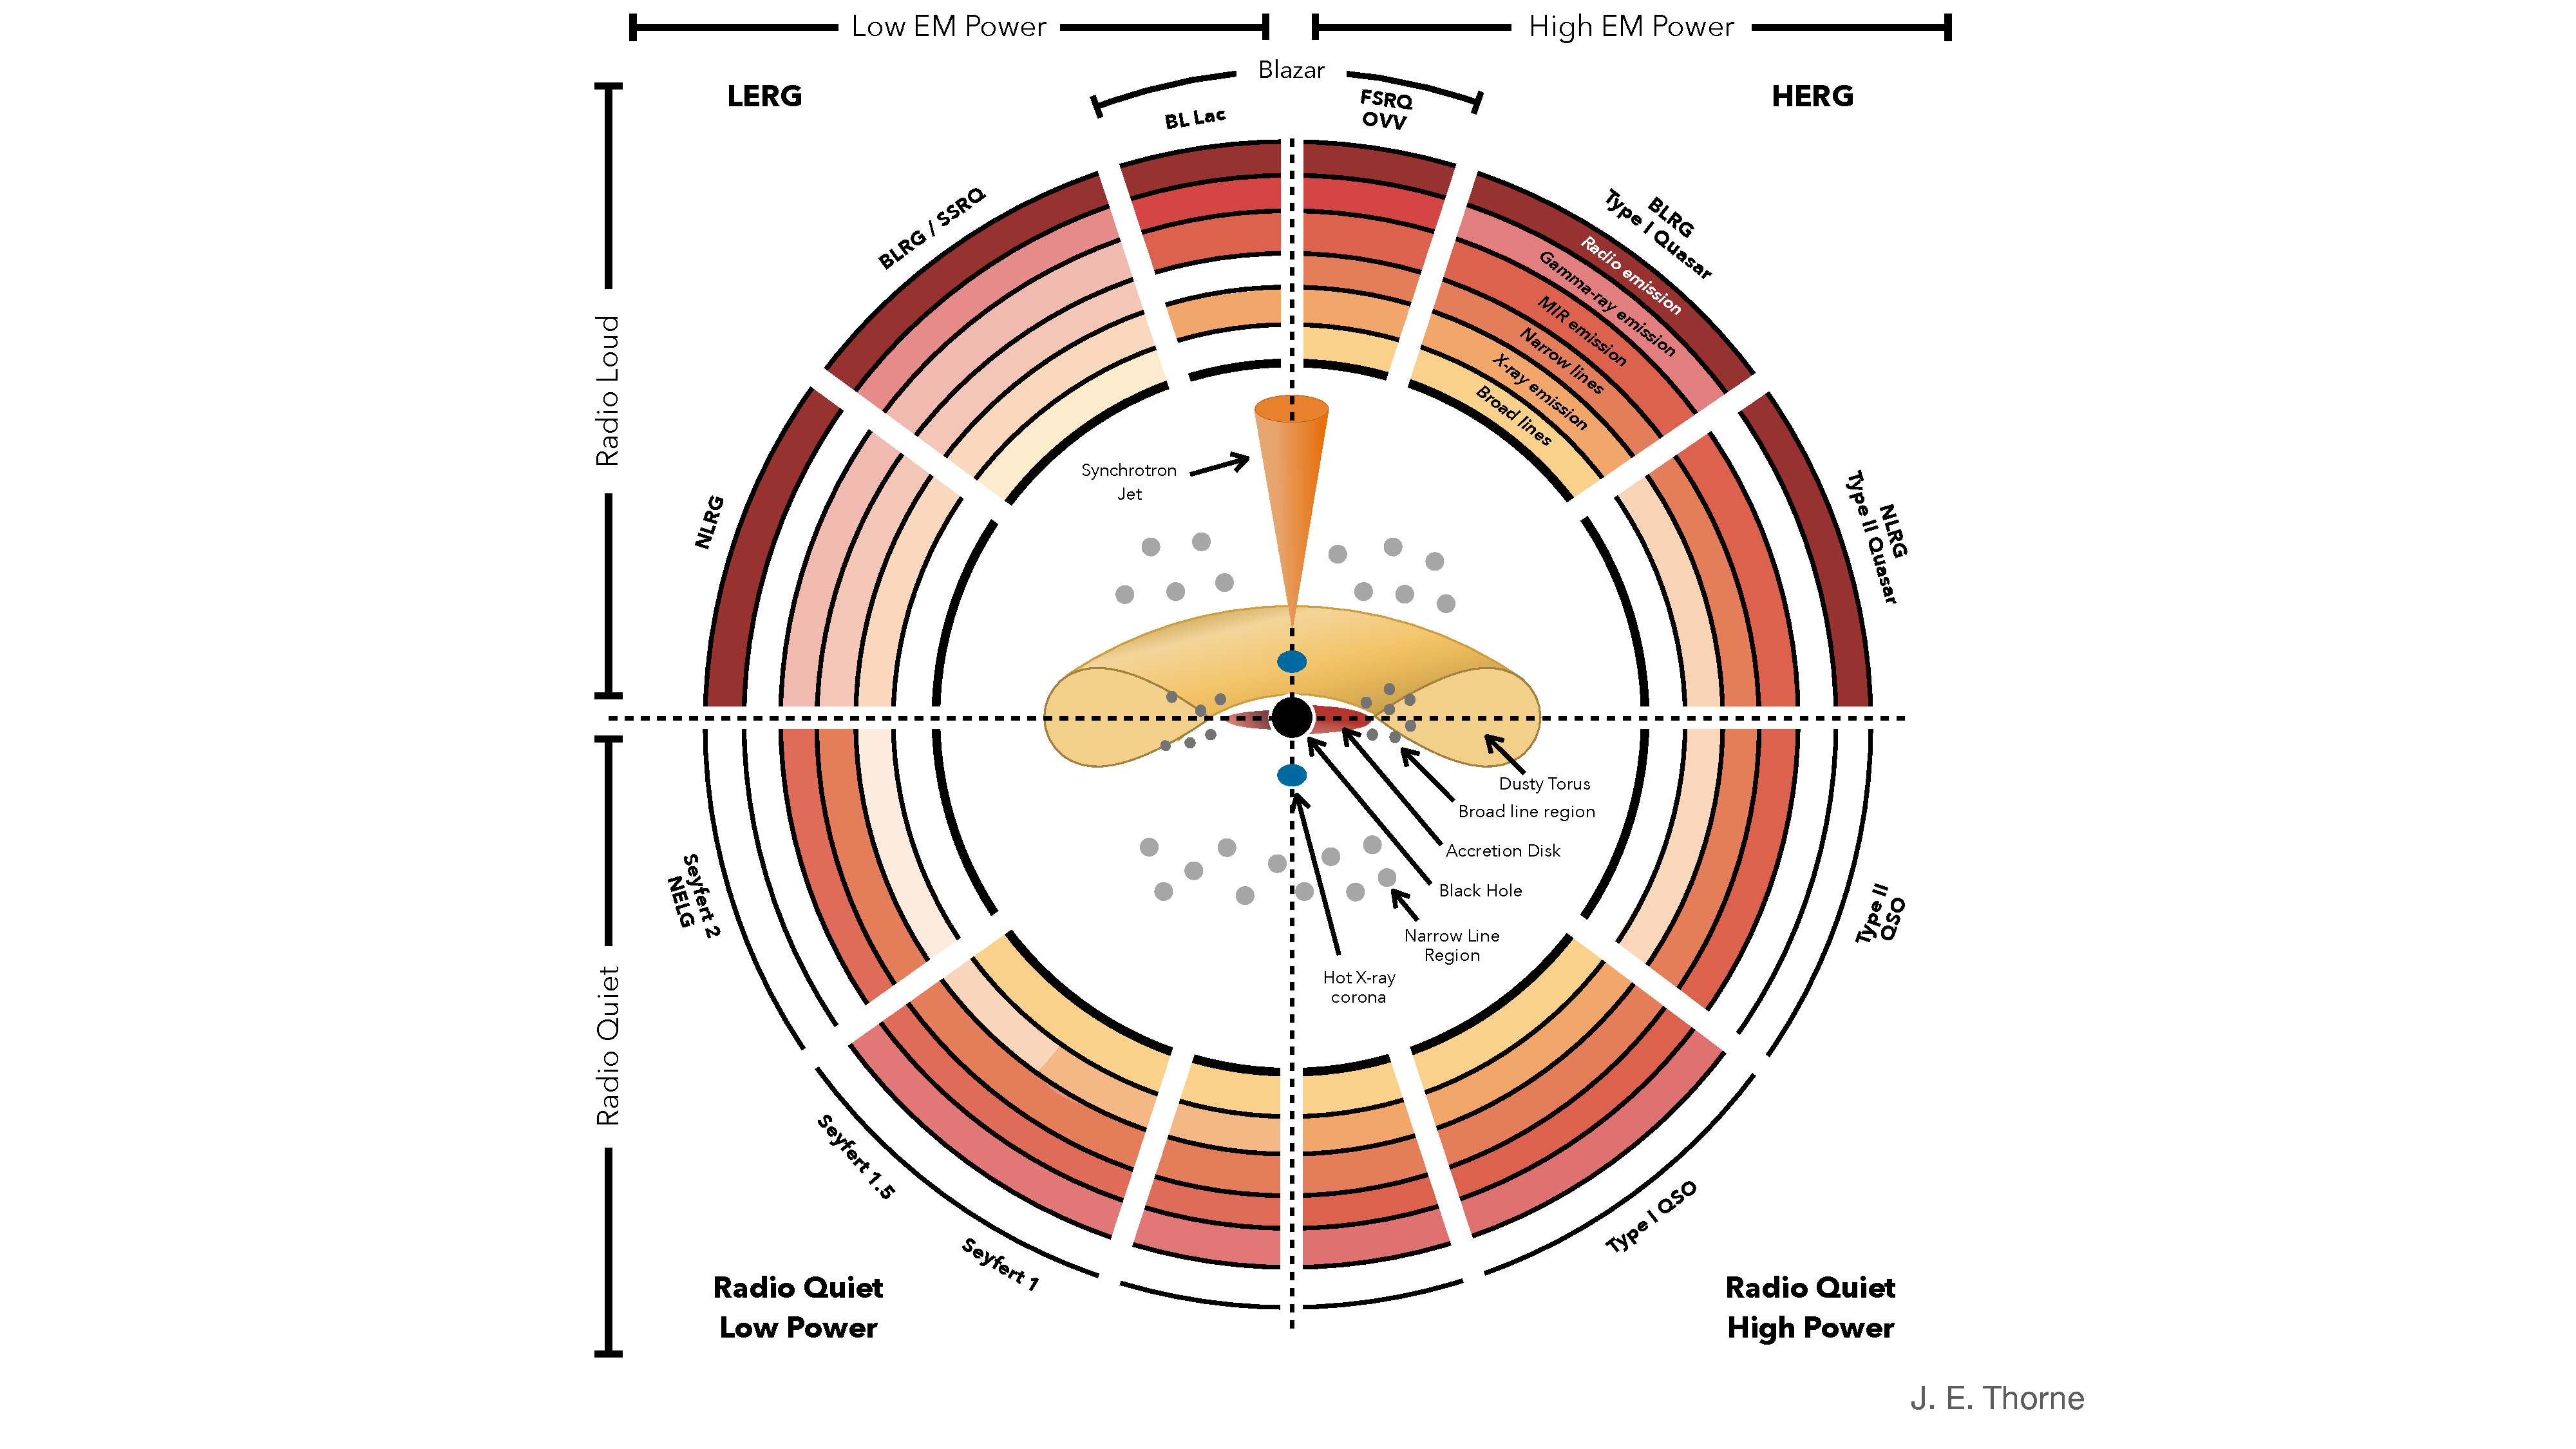
\includegraphics[width=\textwidth]{graphics/agn.pdf}
    \caption{Unified \gls{agn} model showing the different classifications for \glspl{agn}.
    An \gls{agn} is classified by the existence of a relativistic jet, the viewing angle of the observer
    or how bright it is \cite{agn_diagram}.}
    \label{fig:agn}
\end{figure}\glsreset{agn}

Some of the brightest sources of gamma rays in our galaxy are \glspl{snr} such as the Crab Nebular.
The Crab Nebula, in particular, poses as a so-called standard candle with its constant flux of
\gls{hegr}, allowing to test the performance of new experiments and telescopes. Other sources for
gamma rays include \glspl{grb}, Pulsars and \glspl{agn}, the latter being one of the most common types
of extragalactic gamma-ray sources. \glspl{agn} accrete dust and matter in an accretion disk around the
central black hole. The matter gets accelerated by the gravitational force of the black hole and heats
up. While the exact process is not yet fully understood, some accretion disks form a relativistic jet
which, aside from other wavebands, also emits gamma rays via synchrotron
and inverse-Compton scattering processes. \glspl{agn} themselves can be classified depending on the existence
of a relativistic jet, the viewing angle of the observer or how bright they are. \autoref{fig:agn}
shows the different classifications of \glspl{agn}.

Gamma rays can be detected by a variety of experiments, either ground- or space-based. Space-based
experiments like the \gls{fermilat} are usually more sensitive to lower energies, but their performance
is lower for higher energies, as their effective collection area is comparatively small. Ground-based
experiments, however, are more sensitive to higher energies, although they have to rely on the scattering
of secondary particles in \glspl{eas} induced by the primary particle in Earth's atmosphere.
The gamma-ray sky as observed by \gls{fermilat} over a span of
\(\num{12}\) years is shown in \autoref{fig:LAT}.

\begin{figure}
    \centering
    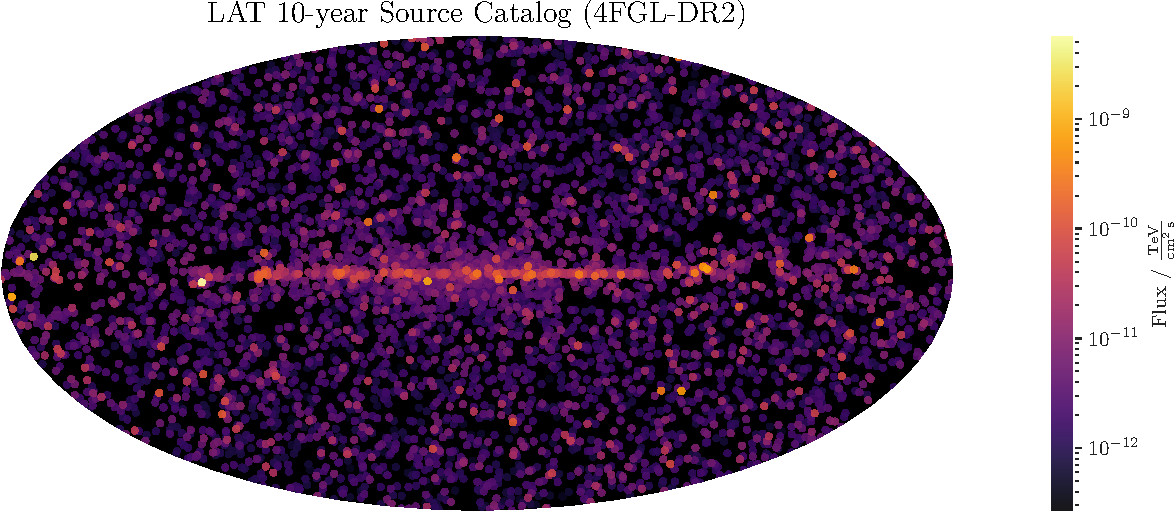
\includegraphics[width=0.8\textwidth]{build/fermi_catalog.pdf}
    \caption{Mollweide projection of the \gls{fermilat} 4FGL-DR3 catalog data of gamma-ray sources. The sky map
    shows the flux of gamma-ray sources in \(\si{\tera\eV\per\centi\meter\squared\per\second}\)
    observed over a span of \(\num{12}\) years from the experiment's launch in 2008. Additionally,
    the Crab Nebula (red circle) is marked along with \glspl{snr} (green circles) and \glspl{agn} (blue circles) that \gls{fermilat}
    observed \cite{fermi4fgl, fermi4fgldr3}. Note the concentration of \gls{he} gamma-ray sources around the galactic plane.}
    \label{fig:LAT}
\end{figure}

For the past two decades, ground-based \gls{iact} experiments like the \gls{magic} telescopes, the
\gls{veritas} and the \gls{hess} have been monitoring these \gls{vhegr} to gain an understanding of
their production. This allowed us to determine different source classes inside and outside our galaxy,
with the most important source class inside our galaxy being \glspl{snr} such as the Crab Nebula.





